% PCCSL 507 Machine Learning Lab - Experiment 4 (NumPy only)
\documentclass[11pt,twoside]{article}

\usepackage[paper=letterpaper,top=0.7in,bottom=0.63in,left=0.75in,right=0.75in,headheight=24pt,headsep=0.14in,footskip=0.38in]{geometry}

\usepackage[T1]{fontenc}
\usepackage{mathptmx} % Times clone
\usepackage{xcolor}
\definecolor{primary}{HTML}{1F3864}
\usepackage{fancyhdr}
\usepackage{array}
\usepackage{colortbl}
\usepackage{parskip}
\setlength{\parindent}{0pt}
\setlength{\parskip}{4pt}
\setlength{\abovedisplayskip}{4pt}
\setlength{\belowdisplayskip}{4pt}
\setlength{\abovedisplayshortskip}{2pt}
\setlength{\belowdisplayshortskip}{2pt}
\usepackage{graphicx}
\usepackage{amsmath}
\usepackage{listings}
\lstset{basicstyle=\footnotesize\ttfamily, breaklines=true, frame=single, showstringspaces=false}

\pagestyle{fancy}
\fancyhf{}
\fancyhead[C]{\textcolor{primary}{\textbf{\small PCCSL 507 Machine Learning Laboratory Record}}}
\renewcommand{\headrulewidth}{0.75pt}
\renewcommand{\headrule}{\hbox to\headwidth{\color{primary}\leaders\hrule height \headrulewidth\hfill}}
\fancyfoot[C]{\footnotesize DEPARTMENT OF CSE \hfill CAPE COLLEGE OF ENGINEERING ALAPPUZHA \hfill Page No. \thepage}
\renewcommand{\footrulewidth}{0pt}

\newcommand{\expheading}[1]{{\fontsize{14}{17}\selectfont\textbf{#1}\par}}
\newcommand{\fullrule}{\noindent\rule{\textwidth}{0.6pt}\par}

\begin{document}
\sloppy

% Sheet-local tightening so it fits one right-side page
{\setlength{\parskip}{1pt}\setlength{\abovedisplayskip}{2pt}\setlength{\belowdisplayskip}{2pt}
\begin{center}
\expheading{EXPERIMENT NO. 4}
\end{center}
\vspace{2pt}

\noindent\textbf{Date:} \underline{\hspace{2.6cm}} \hfill \textbf{Page No.:} \underline{\hspace{2.6cm}}\par
\vspace{6pt}

\expheading{TITLE}
\vspace{4pt}
\noindent NumPy 2D Array -- Branch Sales Analysis\par
\vspace{4pt}

\expheading{OBJECTIVE}
\vspace{2pt}
\fullrule
\vspace{4pt}
\noindent To use a 2D NumPy array for branch sales data and perform indexing, slicing and aggregation to find weekly totals, branch averages, day-wise totals and the top branch. \par
\vspace{4pt}

\expheading{AIM}
\vspace{4pt}
\noindent To store sales data in a 2D array and compute branch/day-wise totals, averages and the highest-selling branch using NumPy. \par
\vspace{4pt}

\expheading{THEORY}
\vspace{4pt}
Sales matrix ($3$ branches $\times$ $7$ days):
\[S=\begin{bmatrix}s_{11} & \cdots & s_{17}\\s_{21} & \cdots & s_{27}\\s_{31} & \cdots & s_{37}\end{bmatrix}\]
Indexing and slicing:
\[S[0],\; S[1,3:],\; S[:,0:3]\]
Weekly total per branch and grand total:
\[W_i=\sum_{j=1}^{7}s_{ij}\quad(\text{axis}=1)\qquad T=\sum_{i,j}s_{ij}\]
Branch average and day-wise total:
\[\bar{B}_i=\frac{1}{7}\sum_{j=1}^{7}s_{ij}\qquad D_j=\sum_{i=1}^{3}s_{ij}\quad(\text{axis}=0)\]
Top branch:
\[k=\arg\max_i W_i\]
\vspace{4pt}

\expheading{PROCEDURE}
\vspace{4pt}
\noindent 1. Store the sales data of 3 branches over 7 days in a 2D NumPy array and display it.\par
\noindent 2. Display the 1st branch sales, Mon--Wed sales and 2nd-branch sales from Thursday.\par
\noindent 3. Find weekly total per branch, grand total, branch-wise average and day-wise total.\par
\noindent 4. Find the branch with the highest sales, display all results and plot the daily-sales bar and pie charts. \par
\vspace{4pt}

\expheading{DATASET DESCRIPTION}
\vspace{4pt}
\noindent Dataset Name: Branch sales (entered in program)\par
\noindent Source: 3 branches $\times$ 7 days (Mon--Sun), synthetic figures\par
\noindent Number of Samples: 21 entries \hspace{0.3cm} Number of Features: 7 days\par
\noindent Target / Class: Not applicable (aggregation operations)\par
\noindent Description: B1=[1200, 1350, 1100, 1450, 1600, 2000, 1800]; B2=[900, 1100, 950, 1200, 1300, 1700, 1500]; B3=[1500, 1600, 1400, 1750, 1900, 2200, 2100]. \par
\vspace{4pt}
} % end sheet-local tightening

\newpage
\expheading{PROGRAM}
\vspace{6pt}

\begin{lstlisting}
import numpy as np
import matplotlib
matplotlib.use("Agg")
import matplotlib.pyplot as plt

days = ["Mon", "Tue", "Wed", "Thu", "Fri", "Sat", "Sun"]

sales = np.array([
    [1200, 1350, 1100, 1450, 1600, 2000, 1800],
    [900, 1100, 950, 1200, 1300, 1700, 1500],
    [1500, 1600, 1400, 1750, 1900, 2200, 2100],
])

print("Complete sales data (branches x days):")
print(sales)

print("1st branch sales =", sales[0])

print("Mon-Wed sales:")
print(sales[:, 0:3])

print("2nd branch from Thursday =", sales[1, 3:])

print("Weekly total per branch =", sales.sum(axis=1))
print("Grand total =", sales.sum())

print("Branch-wise average =", np.round(sales.mean(axis=1), 2))

print("Day-wise total =", sales.sum(axis=0))

top = int(sales.sum(axis=1).argmax())
print("Highest sales: branch", top + 1)
x = np.arange(len(days))
w = 0.25
plt.figure(figsize=(7, 4.5))
plt.bar(x - w, sales[0], width=w, label="Branch 1")
plt.bar(x, sales[1], width=w, label="Branch 2")
plt.bar(x + w, sales[2], width=w, label="Branch 3")
plt.xticks(x, days)
plt.xlabel("Day")
plt.ylabel("Sales")
plt.title("Daily Sales per Branch")
plt.legend()
plt.tight_layout()
plt.savefig("exp4_sales.png", dpi=150)
plt.figure(figsize=(5, 4))
plt.pie(sales.sum(axis=1), labels=["Branch 1", "Branch 2", "Branch 3"], autopct="%1.1f%%")
plt.title("Branch Share of Total Sales")
plt.tight_layout()
plt.savefig("exp4_pie.png", dpi=150)
\end{lstlisting}

\newpage
\expheading{OUTPUT}
\vspace{2pt}
\noindent\rule{\textwidth}{0.5pt}\par
\vspace{4pt}
\begin{verbatim}
Complete sales data (branches x days):
[[1200 1350 1100 1450 1600 2000 1800]
 [ 900 1100  950 1200 1300 1700 1500]
 [1500 1600 1400 1750 1900 2200 2100]]
1st branch sales = [1200 1350 1100 1450 1600 2000 1800]
Mon-Wed sales:
[[1200 1350 1100]
 [ 900 1100  950]
 [1500 1600 1400]]
2nd branch from Thursday = [1200 1300 1700 1500]
Weekly total per branch = [10500  8650 12450]
Grand total = 31600
Branch-wise average = [1500.   1235.71 1778.57]
Day-wise total = [3600 4050 3450 4400 4800 5900 5400]
Highest sales: branch 3
\end{verbatim}
\vspace{4pt}

\begin{center}
\begin{minipage}{0.48\textwidth}\centering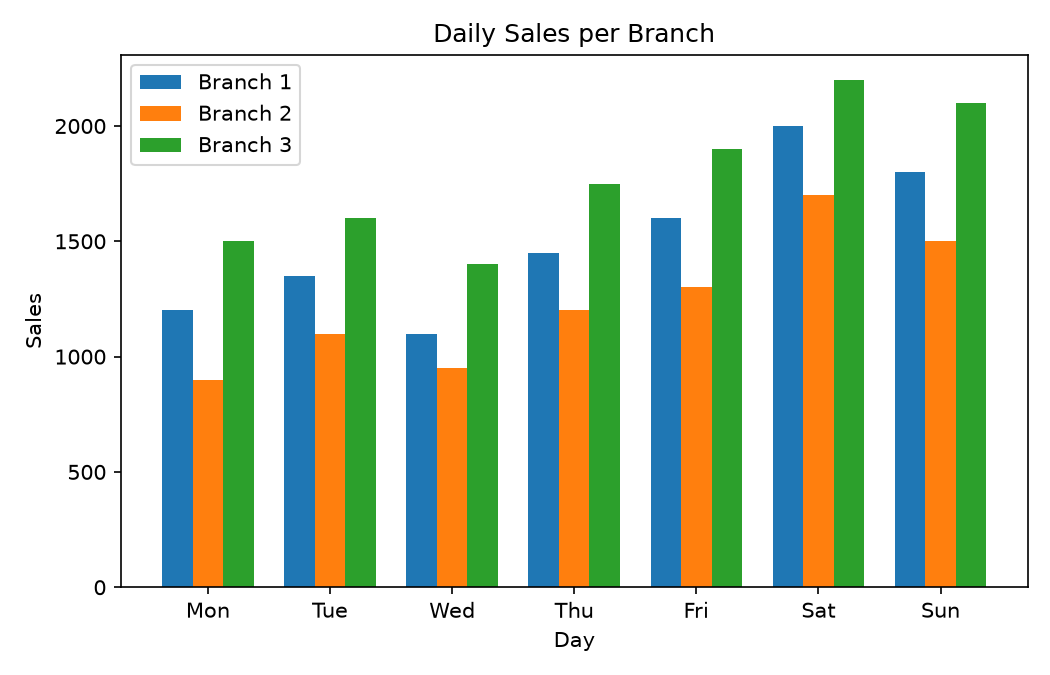
\includegraphics[width=\textwidth]{exp4_sales.png}\par{\small Fig. 1: Daily sales per branch.}\end{minipage}\hfill
\begin{minipage}{0.48\textwidth}\centering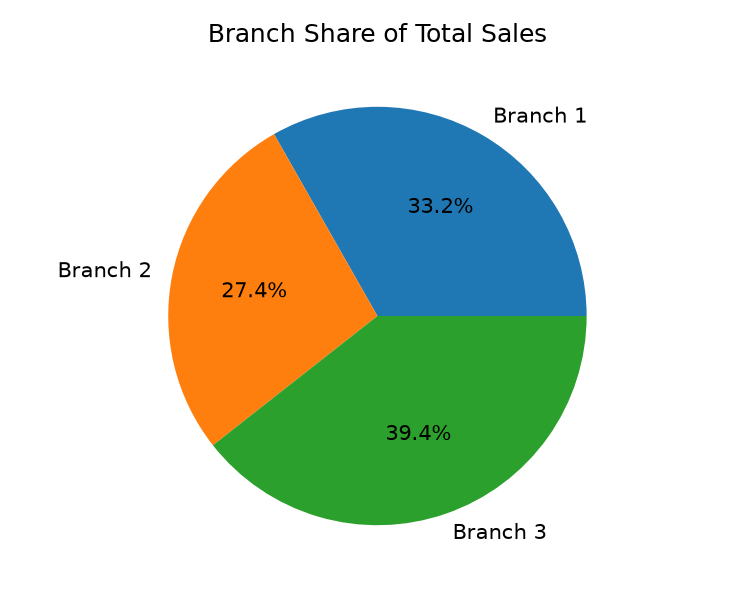
\includegraphics[width=\textwidth]{exp4_pie.png}\par{\small Fig. 2: Branch share of total sales.}\end{minipage}
\end{center}
\vspace{4pt}

\expheading{RESULT}
\vspace{4pt}
{\fontsize{12}{15}\selectfont
The above program was implemented and executed successfully using Python, and the corresponding output was obtained and verified. The results of the \textbf{NumPy data visualization} were analyzed and found to be satisfactory, thereby achieving the desired objective of the experiment.\par
}

\vspace{12pt}

\noindent\textbf{Faculty Signature:} \underline{\hspace{3.6cm}} \hfill \textbf{Date:} \underline{\hspace{2.8cm}}\par

\end{document}
